\documentclass[./\jobname.tex]{subfiles}
\begin{document}

\chapter{Experimental Design}
This chapter gives an overview on how the subsequent experiments are conducted. An integral part of solver comparison is to define a testbed that holds example problems with a known analytical solution. Further, a quality measurement must be defined that compares the numerical to the analytical solution. Since the memory consumption and the solving time is of interest, a robust method to measure these characteristics is needed. The baseline for all experiments is the \gls{fem} solver NGSolve (\cite{schoberl_ngsolvengsolve_2020}). 

\section{Testbed}
\label{chap:testbed_description}
The testbed is a collection of multiple 2-dimensional scalar \gls{pde}s that are analytically solved such that $u(\mathbf{x}): \mathbb{R}^2 \rightarrow \mathbb{R}$ is a solution to the underlying PDE. These can be used to demonstrate the correct implementation of a solver. The testbed can also be used to compare the performance of the classical \gls{fem} solver (NGSolve) with the \gls{ci} solver. The equations and graphs are displayed in the appendix \ref{chap:testbed}. The equations used here are a mixture of different testbeds. Specifically, the equations \gls{pde} 2 and \gls{pde} 3 are picked from the testbed in \cite{chaquet_using_2019}. These problems were also used by \cite{tsoulos_solving_2006} and \cite{panagant_solving_2014}. Preliminary tests have shown that the equations used in these papers are rather simple to approximate. Thus, more complicate equations are added to test the solvability over a wider variety of functions. The more complex equations are taken from the National Institute of Standards and Technology (NIST) website (\cite{mitchell_nist_2018}) that provides benchmarking problems for \gls{fem} solvers with adaptive mesh refinement methods. The other equations 0A, 0B and 8 are specially created to show different properties of the solver. 

\textbf{PDE 0A: Gauss Kernel} \\
\underline{Equation Reference:} \eqref{eq:pde0a} \\
\underline{Characteristics:} sum of 5 \gls{gak}, thus can be approximated arbitrarily close; is designed to show convergence towards analytical solution; \\
\underline{Difficulty:} not especially difficult; \\
\underline{Boundary:} function value of solution; \\

\textbf{PDE 0B: GSin Kernel} \\
\underline{Equation Reference:} \eqref{eq:pde0b} \\
\underline{Characteristics:} can be approximated arbitrarily close by 3 \gls{gsk}; only 3 kernels are used to keep the minimal necessary dimension of the representation similar to \gls{pde} 0A;\\
\underline{Difficulty:} the contrast between a dominant wave with a steep gradient in the middle and small waves with little influence on the boundary; simple approximations lay the focus on the middle, while good approximations also match the small waves; \\
\underline{Boundary:} function value of solution; \\

\textbf{PDE 1: Polynomial 2D} \\
\underline{Equation Reference:} \eqref{eq:pde1} \\
\underline{Characteristics:} polynomial of order 20 \\
\underline{Difficulty:} global structure similar to a \gls{gak}; thus, it should be simple to approximate; \\
\underline{Boundary:} homogeneous boundary condition; \\
\underline{Reference:} \cite{mitchell_nist_2018} \\

\textbf{PDE 2: Chaquet PDE 1} \\
\underline{Equation Reference:} \eqref{eq:pde2} \\
\underline{Characteristics:} compare the performance to other solvers; \\
\underline{Difficulty:} rather simple; slight curvature and no steep gradient; \\
\underline{Boundary:} function value on boundary; \\
\underline{Reference:} \cite{chaquet_using_2019}, \cite{chaquet_solving_2012}, \cite{tsoulos_solving_2006}, \cite{sobester_genetic_2008}, \cite{panagant_solving_2014}\\

\textbf{PDE 3: Chaquet PDE 3} \\
\underline{Equation Reference:} \eqref{eq:pde3} \\
\underline{Characteristics:} compare the performance to other solvers; polynomial of order 2; \\
\underline{Difficulty:} well behaved, no steep gradient; \\
\underline{Boundary:} function value on boundary; \\
\underline{Reference:} \cite{chaquet_using_2019}, \cite{chaquet_solving_2012}, \cite{tsoulos_solving_2006}, \cite{panagant_solving_2014} \\

\textbf{PDE 4: Sine Bump 2D} \\
\underline{Equation Reference:} \eqref{eq:pde4} \\
\underline{Characteristics:} this \gls{pde} is used in both, the work of \cite{chaquet_using_2019} and  \cite{mitchell_nist_2018} with slightly different boundary condition; preliminary test have shown that the \cite{chaquet_using_2019} \gls{pde} is easier to solve, thus this formulation is disregarded;\\
\underline{Difficulty:} sharp boundary condition on the corners of $\Omega$ \\
\underline{Boundary:} homogeneous boundary condition; \\
\underline{Reference:} \cite{mitchell_nist_2018}\\

\textbf{PDE 5: Arctan Circular Wave Front} \\
\underline{Equation Reference:} \eqref{eq:pde5} \\
\underline{Characteristics:} quarter section of slightly shifted arctan; \\
\underline{Difficulty:} transition from the flat plateaus to the steep gradient of the circular wave front; preliminary tests have shown that this problem is especially hard; \\
\underline{Boundary:} function value on boundary \\
\underline{Reference:} \cite{mitchell_nist_2018} \\

\textbf{PDE 6: Peak 2D} \\
\underline{Equation Reference:} \eqref{eq:pde6} \\
\underline{Characteristics:} solution is a single but sharp Gaussian ``peak'' at $(0.5, 0.5)$; \\
\underline{Difficulty:} large negative exponent in e-function results in a steep gradient and small region of interest; \\
\underline{Boundary:} function value on boundary; \\
\underline{Reference:} \cite{mitchell_nist_2018} \\

\textbf{PDE 7: Boundary Line Singularity} \\
\underline{Equation Reference:} \eqref{eq:pde7} \\
\underline{Characteristics:} the solution to this problem is a root function, that is only defined on $x \in \mathbb{R}^{+}$; \\
\underline{Difficulty:} line singularity on boundary with increasing gradient; \\
\underline{Boundary:} function value with singularity on boundary $x_0 = 0$; \\
\underline{Reference:} \cite{mitchell_nist_2018} \\

\textbf{PDE 8: Interior Point Singularity} \\
\underline{Equation Reference:} \eqref{eq:pde8} \\
\underline{Characteristics:} root function; a singularity within the domain; \\
\underline{Difficulty:} not defined at $(0.5, 0.5)$ which results in numerical inaccuracies; \\
\underline{Boundary:} function value on boundary; \\

\textbf{PDE 9: Arctan Wave Front Homogeneous Boundary Conditions 2D} \\
\underline{Equation Reference:} \eqref{eq:pde9} \\
\underline{Characteristics:} arctan oscillation diagonal to the domain;  \\
\underline{Difficulty:} steep gradient on the transition between wave peak and trough; sharp corners on the boundary; \\
\underline{Boundary:} homogeneous boundary condition; \\
\underline{Reference:} \cite{mitchell_nist_2018} \\


\section{Software Architecture}
\label{chap:software_architecutre}

To simplify the preparation, execution and evaluation of the experiments, a comprehensive software architecture is defined. The \gls{uml} class diagram can be seen in the appendix \ref{chap:appendix_software_architecture}. The limited class diagram, without any methods and attributes is shown in the figure \ref{fig:uml_class_small} below. The architecture is organised in 4 main segments. 

\large \underline{\textbf{Optimisation Algorithm}} \\
The \inlinecode{IOptAlgoBase} interface must be implemented by every \inlinecode{OptAlgo} class to ensure the compatibility with \inlinecode{CiPdeBase} class of the testbed. A nice side-effect is that it reduces the number of user-defined parameters. An optimisation algorithm of this class must only take an initial guess (e.g. the starting population) as well as two stopping criteria: the maximum number of function evaluation or a minimum error to reach. Also a fitness function (i.e. the function to be optimised) must be provided. Four lists of the same length are returned: the optimum-guess, the function value, the crossover probability and the scale factor per each generation. The actual implementation of the algorithm is not predefined. 

\large \underline{\textbf{Kernels}} \\
As described in chapter \ref{chap:candidate_rep}, a candidate solution is defined as a sum of \gls{rbf}. In order to test different candidate representations, different classes must be implemented. Again, to ensure compatibility with the \inlinecode{CiPdeBase} class, all representations must implement the \inlinecode{IKernelBase} interface. This assures that all classes have a method that can calculate the solution as well as the first and the second order derivatives. Here, only two kernels are implemented. A typical Gauss kernel as described in chapter \ref{chap:gauss_kernel} and a so called GSin kernel shown in chapter \ref{chap:gsin_kernel}. 

\large \underline{\textbf{Testbed}} \\
The testbed holds the 11 differential equations used in all experiments. The testbed is abstracted in such a way that an experiment is as simple as creating an \gls{pde} object and calling its solve method. All testbed classes must implement the \inlinecode{ITestbenchBase} interface. This ensures the minimal functionality of every subsequent class. Currently two classes implement this interface, the \inlinecode{FemPdeBase} and the \inlinecode{CiPdeBase}. These are the base classes that provide the specific attributes and methods needed for the \gls{fem} solver and the \gls{ci} solver. The actual \gls{pde} problems are implemented in the classes \inlinecode{FemPde0} or \inlinecode{CiPde0} which inherit from the \inlinecode{FemPdeBase} and the \inlinecode{CiPdeBase}, respectively. The number in their name is representative for all different testbench problems and every \gls{pde} has its own class. Since all \gls{pde} classes have the same methods/attributes and only differ in their implementation and name, they do not have to be displayed separately. Therefore, they are symbolised together by a ``stacked notation'' used in the class diagram. Some methods in these classes must be overridden and adapted to the current \gls{pde} problem, which is indicated by the $\land$ character.

\large \underline{\textbf{Post Processing}} \\
Although the post processing block is not actually a class, it is still represented in this diagram. This module provides functions that take \inlinecode{FemPdeN} or \inlinecode{CiPdeN} objects and perform actions with them. The methods are used in the experiments chapters to interpret the results. A detailed description of the implementation is given in the appendix \ref{chap:apendix_post_proc}.

\begin{figure}[H]
	\centering
	\noindent\adjustbox{max width=\linewidth}{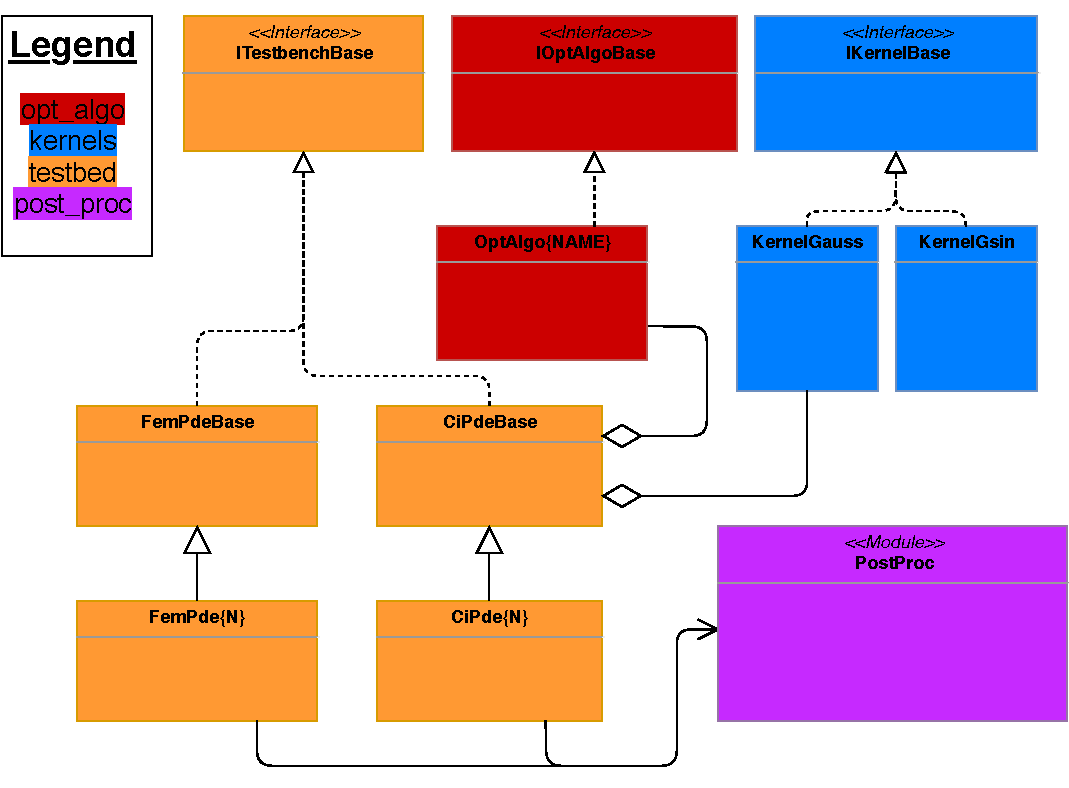
\includegraphics[width=1\textwidth]{../../code/uml_diag/testbench_uml_class_small.pdf}
	}
	\unterschrift{This reduced \gls{uml} class diagram gives an overview of the testbed design and its interfaces and classes.}{}{}
	\label{fig:uml_class_small}
\end{figure}

\section{Performance Metric} 
\label{chap:metric}
In order to scientifically compare the results produced by the different solvers, some metrics are necessary. Three important solver-properties are measured: the execution time, the memory usage and the quality of the numerical solution. The following chapters describe the measurement process in greater detail. 

\subsection{Solving Time}
\label{chap:metric_time}
The solving time is measured within the \inlinecode{solve()} method of either class. The time module of the \cite{python_standard_library_time_2020} is used to interact with the system clock. The resolution, that the time module can access, depends on the system it is running on. Specifically, on the machine used in all further experiments, \inlinecode{time.time()} returns a 24 byte float that represents the time passed since 1st of January 1970. Usually, consecutive calls of this function return increasing values - changing the system time could interfere with the correctness of this value.\\ 

As the execution time of a program depends on many other factors, such as the current system load, the CPU temperature and the process scheduler, it is necessary to view it as a random variable. Thus, multiple replications have to be done before trying to interpret the results. To make for a fair comparison, the same machine with a similar work-load must be used.  The replications are not done within the \inlinecode{solve()} function and must be applied during the experiment. To reduce the random effects and prevent possible outlier, the Python garbage collector is switched off during the time measurement. For a step-by-step description, the pseudocode is displayed in the appendix \ref{chap:solve_function}. 



\subsection{Memory Usage}
\label{chap:metric_mem}
Similar to the solving time measurement, the memory usage is determined within the \inlinecode{solve()} method. The \textit{psutil} module (\cite{rodola_psutil_2020}) provides the functionality to read the amount of memory attached to a process at a given time. The function call \inlinecode{process.memory_info()} returns an object with multiple attributes about the current state of the process. Of special interest is the \gls{vms} field. This includes the \gls{rss}, the memory that is currently held within the main memory, and the memory that is currently swapped out to the hard drive.

Without assuming anything about the inner workings of the process, the memory usage is also a random variable. Thus, similar to the time measurement, replications have to be performed. The same pseudocode as for the time measurement (appendix \ref{chap:solve_function}) also applies here. To remove outliers, it is helpful to create and solve one testbed object before recording the experiment. This sets up the necessary references and then are mingled into the actual solving process. This holds true for both, the \gls{fem} and the \gls{ci} solver.  

\subsection{Quality Measurement}
\label{chap:metric_quality}
Although the fitness function is the criterion that is optimised, it is not applicable as an objective quality measure. As \cite{chaquet_using_2019} describe, it depends on multiple factors:
\begin{itemize}
	\item user-defined parameters $\xi$ and $\phi$ 
	\item the formulation of the \gls{pde} 
	\item number of collocation points used 
	\item number of kernels used
\end{itemize}
Thus, \cite{chaquet_using_2019} define a new quality measurement based on the \gls{rmse} over the collocation points as seen in equation \eqref{eq:rmse_chaquet}. 
\begin{equation}
\label{eq:rmse_chaquet}
RMSE^2 = \frac{\sum_{i=1, \mathbf{x}_i \in C}^{n_C} \left|\left| u(\mathbf{x}_i) - u_{ext}(\mathbf{x}_i) \right|\right|^2 + \sum_{j=1, \mathbf{x}_j \in B}^{n_B} \left|\left| u(\mathbf{x}_j) - u_{ext}(\mathbf{x}_j) \right|\right|^2}{(n_C + n_B)}
\end{equation}
This quality criterion has three inherent issues. At first, it firmly depends on the number of collocation points used. In an algorithm that uses self-adaptive collocation points, where the distribution of the points depends on random variables, subsequent measures of similar solutions could result in different quality values. Especially in solutions with high condition numbers, the \gls{rmse} measurement would be rendered useless since a small deviation of the point results in a large difference of the function value. 

Further with the \gls{rmse}, the quality is only measured on the collocation points and not in between. However, a good solution fits not only these discrete points, but the whole domain. This is called an aliasing error. An approximation can fit the points, without correctly representing the space between them. This is shown in the following figure \ref{fig:aliasing error}.

\begin{figure}[H]
	\centering
	\noindent\adjustbox{max width=0.8\linewidth}{
		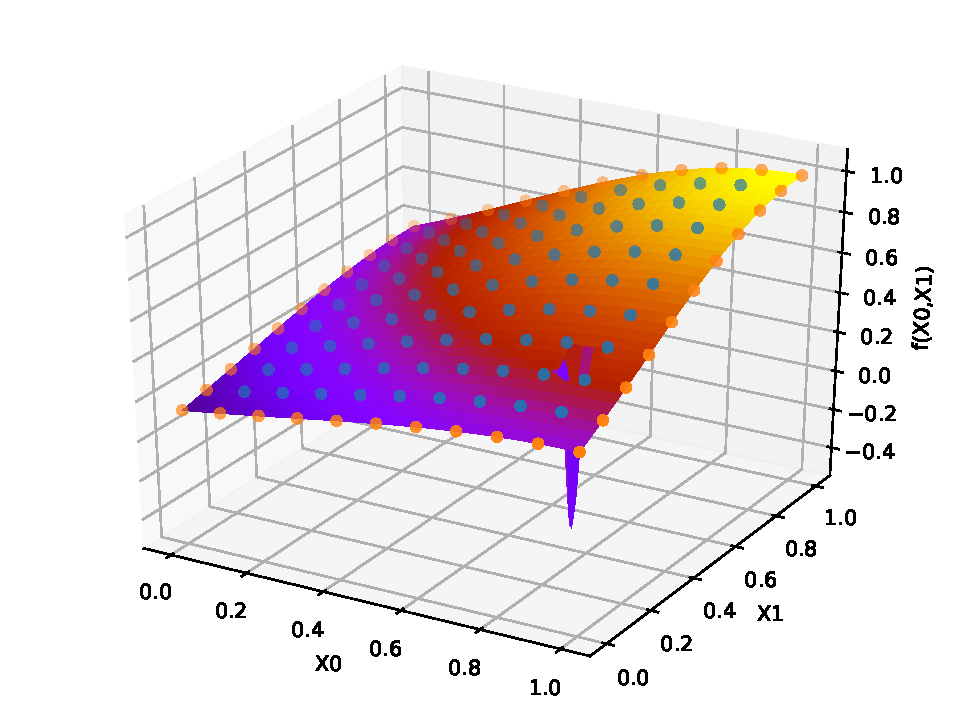
\includegraphics[width=\textwidth]{../img/pdf/aliasing_error.pdf}
	}
	\unterschrift{Aliasing Error: sharp inaccuracies in between collocation points}{}{}
	\label{fig:aliasing error}
\end{figure}

Finally, the \gls{fem} method doesn't use collocation points, so this quality measurement could not be calculated. A good quality measurement tool only uses the numerical and analytical solution, independently of the solving method. 

This leads to the quality measurement formulation used in this thesis: the L2 norm defined for functions as denoted in equation \eqref{eq:quality_measurement}. This actually measures the distance between the analytical solution and the numerical approximation.  
\begin{equation}
\label{eq:quality_measurement}
\left|\left|u_{ext} - u_{apx}\right|\right| = \sqrt{\int_{\Omega} (u_{ext}(\mathbf{x}) - u_{apx}(\mathbf{x}))^2 dx}
\end{equation}
Although this integral is numerically evaluated, the discretisation is much finer than the resolution of the collocation points used in the fitness function - thus also regarding the areas between these points.



\section{Baseline: NGSolve}
\label{chap:fem_baseline_results}
As mentioned above, the NGSolve framework (\cite{schoberl_ngsolvengsolve_2020}) is used as the baseline for all experiments. NGSolve is a state of the art \gls{fem} solver, that is in part developed and maintained by numerous well-known institutes such as Vienna University of Technology, University of Göttingen and Portland State University. This chapter describes the results obtained by running NGSolve on the testbed. The metrics from chapter \ref{chap:metric} are applied. 

\subsection{Setup}
At first the \gls{pde}s must be transformed into their corresponding weak form. As all testbed problems are Poisson equations and only differ in their algebraic sign and inhomogeneous part, the weak form is similar for all problems. Referring to equation \eqref{eq: weak form}, the terms $\vec{b} = 0$ and $c = 0$, thus these parts vanish. The matrix $A$ is either $\begin{bsmallmatrix} 1 & 0 \\ 0 & 1 \end{bsmallmatrix}$ or with a negative sign $\begin{bsmallmatrix} -1 & 0 \\ 0 & -1 \end{bsmallmatrix}$ as only the non-mixed second order derivatives occur in the equations. This results in weak form as presented in equation \eqref{eq: weak form testbed}, where the f is the inhomogeneous part of the \gls{pde}.
\begin{equation}
\label{eq: weak form testbed}
\int_{\Omega} \nabla u^T \nabla v dV = \int_{\Omega} f v dV
\end{equation}

To enhance the performance of NGSolve, static condensation is turned on. Further, a multigrid preconditioner is used. All problems are approximated by second order polynomials. The automatic mesh refinement is performed until a maximum of $5 \cdot 10^4$ \gls{dof} is reached. To properly interpret the results, 20 replications for each problem are performed. This is only needed for regarding time and memory, the solution itself is not a random variable. To further reduce the memory consumption, the GUI of NGSolve is switched off. 

\subsection{Result}
With the parameters described above, the following results are produced. The solving time as well as the memory usage are displayed in the boxplots \ref{fig:_fem_time_boxplot} and \ref{fig:_fem_mem_boxplot}, respectively. These datasets provide a reference point for the performance of the \gls{ci} solver. In general, the solving time ranges from 2.5 to 5.0 seconds at about 50 to 80 Mbyte of memory. Only problem 3 stands out as a notable exception. To keep the diagram within a readable scale, this \gls{pde} is omitted and plotted in a separate figure. 

Table \ref{tab:fem_sol_quality} presents the achieved distances between the exact and the approximated solutions. On \gls{pde} 3 the best numerical quality is achieved.

The problem \gls{pde} 7 only needs around 2.5 seconds to be solved. A reason could be that the solution only depends on one variable and the derivative with respect to y $\frac{\partial u}{\partial y} = 0$ vanishes. This does not effect the memory usage, since all $5 \cdot 10^4$ \gls{dof} must be created to terminate. 

\begin{table}[h]
	\centering
	\noindent\adjustbox{max width=\linewidth}{
		\begin{tabular}{|c|c|}
			
			\hline
			\rowcolor[HTML]{\farbeTabA}
			
			Problem PDE & L2 Norm \\ \hline
			
			0A & $2.967 \cdot 10^{-5}$ \\ \hline
			0B & $1.071 \cdot 10^{-5}$ \\ \hline
			1  & $8.004 \cdot 10^{-7}$ \\ \hline
			2  & $3.501 \cdot 10^{-8}$ \\ \hline
			3  & $1.680 \cdot 10^{-9}$ \\ \hline
			4  & $4.764 \cdot 10^{-7}$ \\ \hline
			5  & $6.057 \cdot 10^{-6}$ \\ \hline
			6  & $1.908 \cdot 10^{-7}$ \\ \hline
			7  & $5.203 \cdot 10^{-5}$ \\ \hline
			8  & $3.237 \cdot 10^{-7}$ \\ \hline
			9  & $2.366 \cdot 10^{-7}$ \\ \hline
			
		\end{tabular}
	}
	\unterschrift{These are the results obtained by the \gls{fem} solver in terms of distance to the analytical solution. The solver achieves the smallest deviation in PDE 3.}{}{}
	\label{tab:fem_sol_quality}
\end{table}


\begin{figure}[H]
	\centering
	\noindent\adjustbox{max width=0.66\linewidth}{
		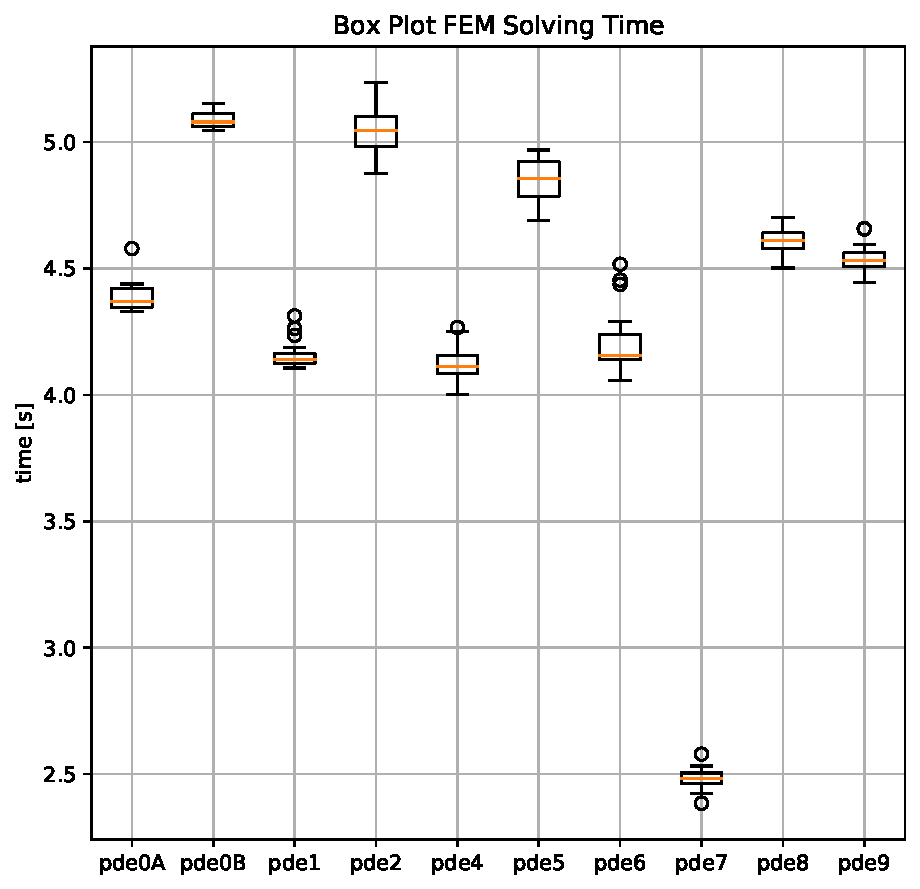
\includegraphics[width=\textwidth]{../../code/experiments/_experiment_fem_base/time_boxplot_pde_0a_0b_1_2_4_5_6_7_8_9.pdf}
	}
	\unterschrift{Boxplot: time (in seconds) needed to solve the testbed \gls{pde} (without \gls{pde}3)}{}{}
	\label{fig:_fem_time_boxplot}
\end{figure}

\begin{figure}[H]
	\centering
	\noindent\adjustbox{max width=0.66\linewidth}{
		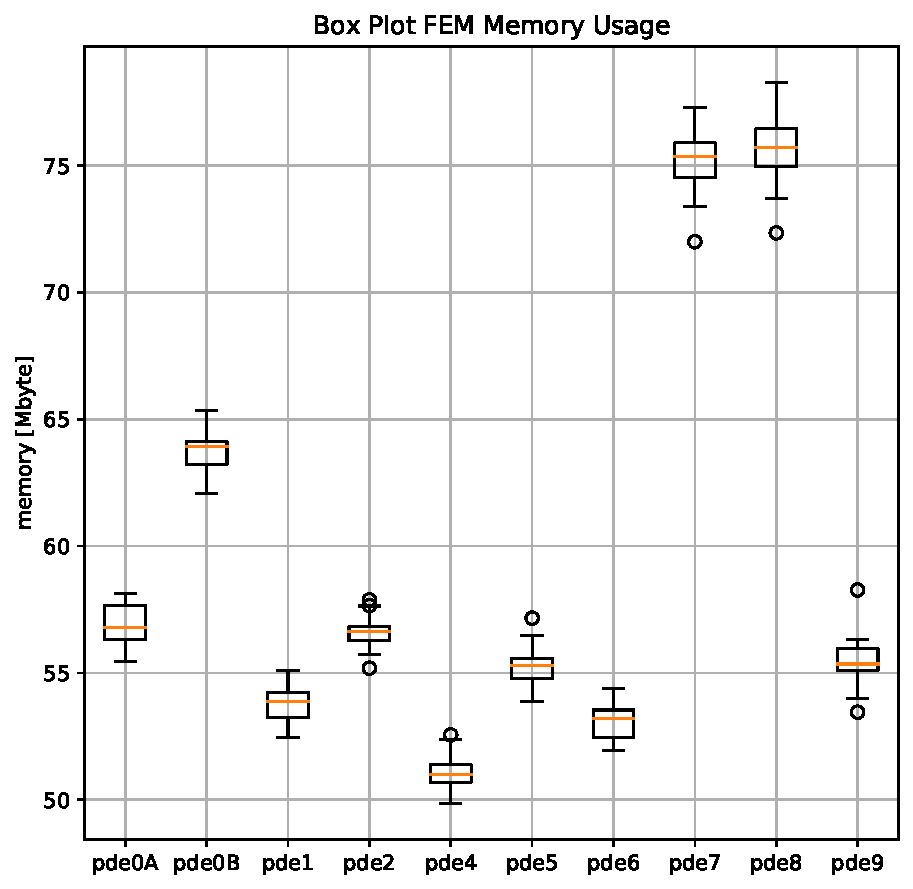
\includegraphics[width=\textwidth]{../../code/experiments/_experiment_fem_base/mem_boxplot_pde_0a_0b_1_2_4_5_6_7_8_9.pdf}
	}
	\unterschrift{Boxplot: memory (in Mbyte) needed to solve the testbed \gls{pde} (without \gls{pde}3)}{}{}
	\label{fig:_fem_mem_boxplot}
\end{figure}

The following figures \ref{fig:_fem_time_boxplot_pde3} and \ref{fig:_fem_mem_boxplot_pde3} show the boxplot of the time and memory consumption for the testbed \gls{pde} 3 with $5 \cdot 10^4$ \gls{dof}. Compared to the other equations, this problem takes longer to solve while also needing more memory: somewhere around 65.2 seconds at about 130 Mbyte. One possible explanation for that is the fundamental structure of the \gls{pde}. As described in equation \eqref{eq:sol3}, the exact solution to this problem is a polynomial of second order. This can be approximated perfectly by the \gls{fem} solver, since it also uses second order polynomials as basis functions. The mesh-refinement step takes more iterations to produce the $5 \cdot 10^4$ \gls{dof} as compared to the other testbed problems. In fact, since the numerical errors per finite element accumulate, more \gls{dof} should result in a larger approximation error. Figure \ref{fig:_dof_sweep_pde3} shows the performance metrics at different \gls{dof} budgets. The plot confirms this hypothesis, that less \gls{dof} take less time and memory to solve the \gls{pde} and still end up with a better quality. 

\begin{figure}[H]
	\centering
	\noindent\adjustbox{max width=0.7\linewidth}{
		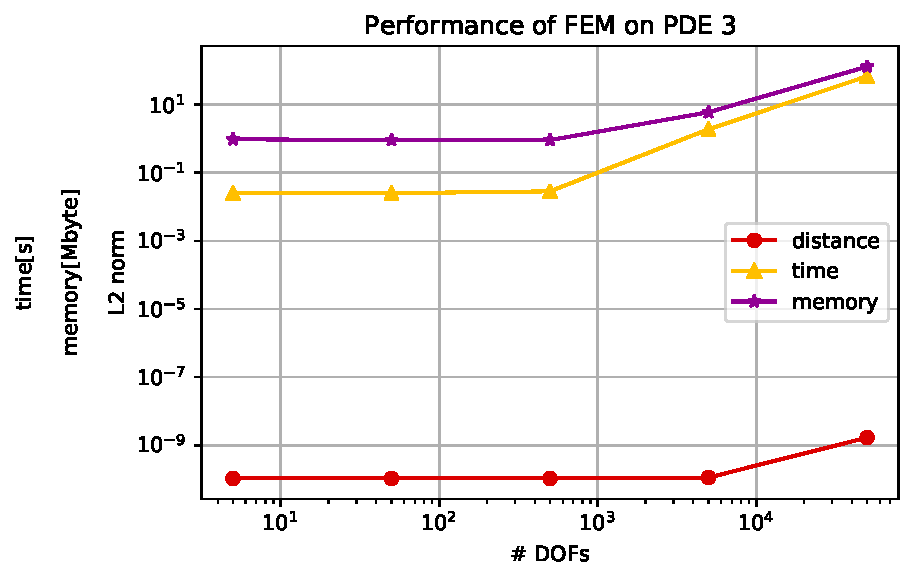
\includegraphics[width=\textwidth]{../../code/experiments/_experiment_fem_base/pde3_ndof.pdf}
	}
	\unterschrift{\gls{pde} 3 performance metrics at different \gls{dof} budgets.}{}{}
	\label{fig:_dof_sweep_pde3}
\end{figure}

\begin{figure}[H]
	\centering
	\begin{subfigure}[b]{0.5\linewidth}
		\centering
		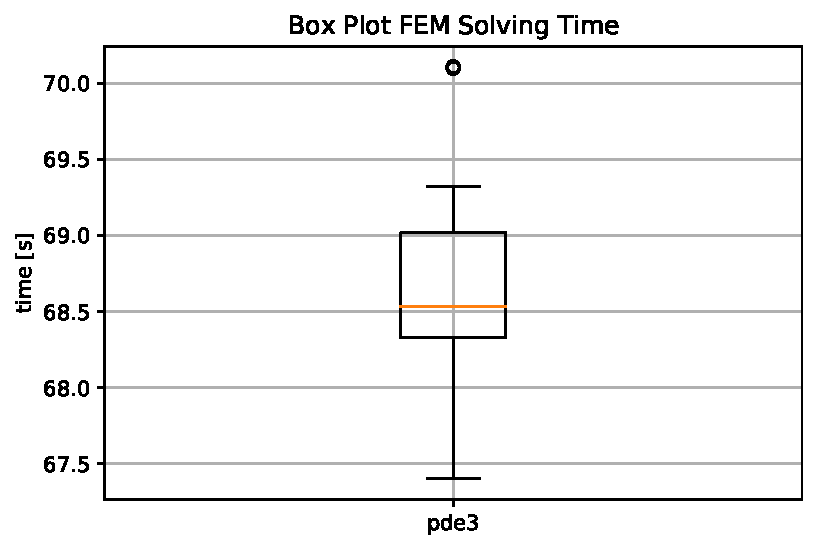
\includegraphics[width=1\textwidth]{../../code/experiments/_experiment_fem_base/time_boxplot_pde_3.pdf}
		\caption{Boxplot: time to solve testbed \gls{pde}3 at $5\cdot 10^4$ \gls{dof}.}
		\label{fig:_fem_time_boxplot_pde3}
	\end{subfigure}% 
	%
	\begin{subfigure}[b]{0.5\linewidth}
		\centering
		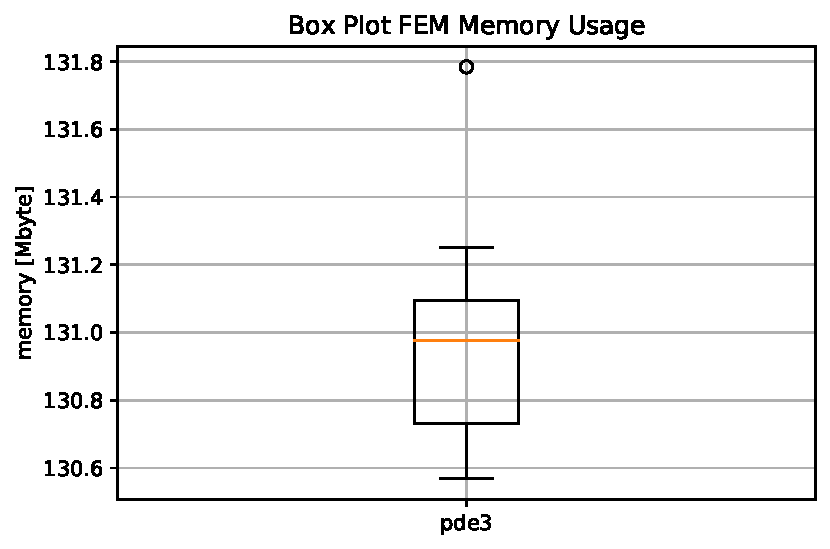
\includegraphics[width=1\textwidth]{../../code/experiments/_experiment_fem_base/mem_boxplot_pde_3.pdf}
		\caption{Boxplot: memory to solve testbed \gls{pde}3 at $5\cdot 10^4$ \gls{dof}.}
		\label{fig:_fem_mem_boxplot_pde3}
	\end{subfigure}%
	\unterschrift{Comparison of time and memory effort on \gls{pde} 3 at $5 \cdot 10^4$ \gls{dof}.}{}{}%
	\label{}
\end{figure}

\section{Default CI Parameter}
\label{chap:default_ci_param}
Typically, the performance of heuristic optimisation algorithms can be adjusted to specific testbed problems by tuning its parameters. For all further experiments the JADE algorithm from pseudocode \ref{algo: jade} is used. Similarly, the reported \gls{ci} solver has many parameters that could be adapted. However, adjusting every parameter in order to find the best combination is not an option, since that would take an extensive amount of computation time. Some parameters that might not have a great effect on the performance can be predefined. These values are determined by preliminary test. If not stated otherwise, the following parameters from table \ref{tab:ci_parameter} are used in the subsequent experiments. 

\begin{table}[h]
	\centering
	\noindent\adjustbox{max width=\linewidth}{
		\begin{tabular}{|c|c|c|}
			
			\hline
			\rowcolor[HTML]{\farbeTabA}
			
			Parameter & JADE & \multilinecell{\gls{cma_es} \\ (\cite{chaquet_using_2019})} \\ \hline
			
			$\varphi$ & 100 & 300 \\ \hline
			$\kappa$  & 1   & 3   \\ \hline
			population size & $2 \cdot dim$ & $\frac{3}{2}(4 + \lfloor 3 \cdot ln(dim) \rfloor)$ \\ \hline
			min error & 0   & - \\ \hline
			p & 0.3 & - \\ \hline
			c & 0.5 & - \\ \hline
			replication & 20 & 50 \\ \hline
			\multilinecell{nb \\ nc \\~\\ } & \multilinecell{40 \\ 81 \\ \hline 121 = 11x11}  & \multilinecell{100 equally spaced \\ points over the domain} \\ \hline
			initialisation & $\vec{u_{apx}} \in \mathcal{N}(0,1)$ & \multilinecell{$\omega_i \in \mathcal{U}[-0.01, 0.01]$ \\ $\gamma_i \in \mathcal{U}(0,1]$ \\ $c_{ik} \in \mathcal{U}[2\Omega]$}  \\ \hline
			
		\end{tabular}
	}
	\unterschrift{These predefined parameters are used for the following numerical experiments. }{}{}
	\label{tab:ci_parameter}
\end{table}

The parameters $\varphi$ and $\kappa$ are used in the fitness function (equation \eqref{eq:fit_func}) for changing the relative importance of the boundary and the interior. \cite{chaquet_using_2019} take similar values. However, preliminary tests have shown, that the current values perform slightly better on the present testbed. Figure \ref{fig:collocation_weight} shows the values of $\xi$ and $\varphi$. It further describes how the weighting factor emphasises the areas closer to the boundary. 

\begin{figure}[h]
	\centering
	\noindent\adjustbox{max width=0.8\linewidth}{
		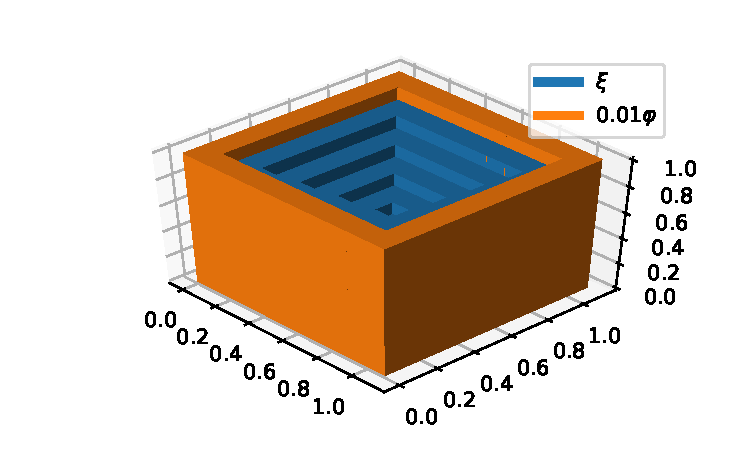
\includegraphics[width=\textwidth]{../img/pdf/collocation_weight.pdf}
	}
	\unterschrift{Weighting factor $\varphi$ and $\xi$ on every collocation point}{}{}
	\label{fig:collocation_weight}
\end{figure}

The population size used by \cite{chaquet_using_2019} is based on the original formulation of the \gls{cma_es}. However, they observed a better convergence when scaling the recommended population size by 3. Typically, \gls{de} uses larger population sizes. \cite{mallipeddi_empirical_2008} describe an empirical study on choosing this parameter. They discuss the trade-off between premature convergence and computational effort. The results suggest that population sizes of $2\cdot dim$ are more likely to stagnate, but also converge faster. Since time is a critical resource, this population size is chosen. 

The termination condition for \gls{de} is either a maximum number of function evaluation, or a minimal function value to reach. Since the fitness function (equation \eqref{eq:fit_func}) has its optimum at 0, this value is used as the termination condition. A helpful side-effect is that it ensures the same amount of function evaluation in every run, without early termination. This prevents outliers in the time and memory measurement. 

The parameters p and c are specific to JADE (algorithm \ref{algo: jade}). The mutation operator \inlinecode{mutationCurrentToPBest1} uses p to select the best individuals and c weights the parameter adaption mechanism. For all experiments these values are set at $p=0.3$ and $c=0.5$. 

To account for the statistical influence, every setup is reevaluated by 20 replications where each replication starts with independent initial guesses. 

\cite{chaquet_using_2019} use 100 equally spaced collocation points over the domain to solve the \gls{pde}. Here, 121 points are created, as seen in figure \ref{fig:collocation_points}. 


\begin{figure}[h]
	\centering
	\noindent\adjustbox{max width=0.6\linewidth}{
		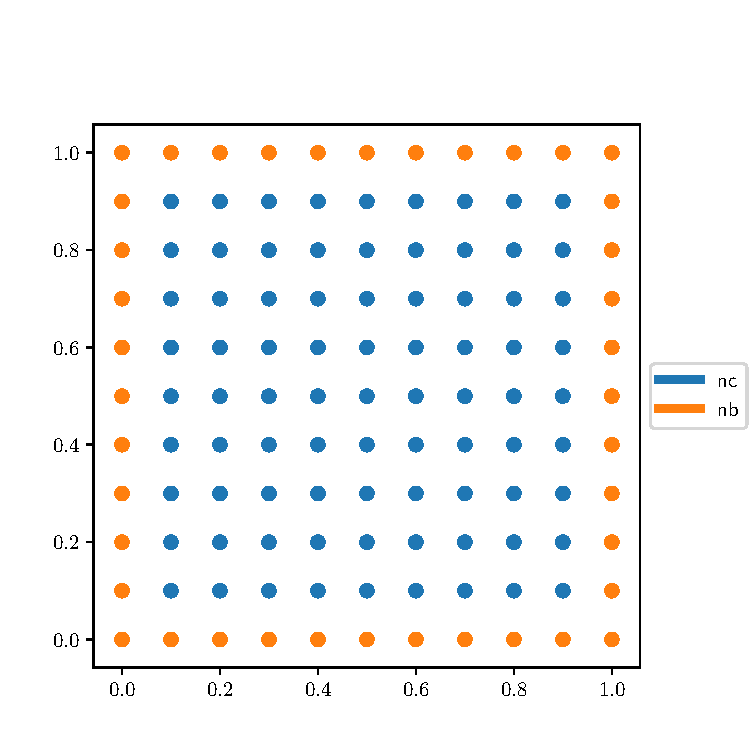
\includegraphics[width=\textwidth]{../img/pdf/testbed_small_domain.pdf}
	}
	\unterschrift{Collocation points used in the testbed. For the \gls{pde}s 0A and 0B with the larger domain, the lower limits $x_0$L and $x_1$L are replaced with -2 and the upper limits $x_0$U and $x_1$U are replaced with 2. The points are still equally spaced.}{}{}
	\label{fig:collocation_points}
\end{figure}

The initialisation is done by a standard normal distribution. This means that every value in the $\mathbf{p_{apx}}$ vector is drawn from a normal distribution. On the contrary, \cite{chaquet_using_2019} initialise the values specifically tailored to each parameter of the kernel. This process assumes a priori information about the solution. In the typical application, this knowledge is not available and thus it should not be used. 


\section{Hardware Infrastructure}
\label{chap:hardware_setup}

To increase the experimental throughput, two machines are used: a personal computer (machine 1) and a server in the cloud (machine 2). It is important that any time or memory comparisons must be performed between experiments on the same machine. In the experiments chapter it is separately denoted which comparisons are allowed. The following table \ref{tab:machines} shows the properties of both machines. It is important to note that these information are only a reference point. This is probably not enough to actually recreate the exact time or memory data presented in this work. 

\begin{table}[h]
	\centering
	\noindent\adjustbox{max width=\linewidth}{
		\begin{tabular}{|c|c|c|}
			
			\hline
			\rowcolor[HTML]{\farbeTabA}
			
			Property & Machine 1 & Machine 2 \\ \hline
			
			Operating System & Windows 10 Home 1909 18363.900 & CentOS Linux release 7.3.1611 \\ \hline
			Python & Anaconda version 2019.03 & Anaconda version 2020.02 \\ \hline
			Processor & Intel Core i7-4790K CPU @ 4.00GHz & Intel Xeon CPU E5-2630 v3 @ 2.40GHz \\ \hline
			Cores & 4 Cores + 4 logical & 32 Cores \\ \hline
			
		\end{tabular}
	}
	\unterschrift{Comparison of the machines used for the experiments.}{}{}
	\label{tab:machines}
\end{table}

Due to the Python incompatibilities, NGSolve can only be installed on machine 1. Thus, any time or memory comparisons between the \gls{ci} solver and the \gls{fem} solver must be done within machine 1. 

\end{document}